\documentclass[12pt]{article}

% All the packages used.
\usepackage[margin=1.0in]{geometry}
\usepackage{pbox}
\usepackage{array}
\usepackage{multicol}
\usepackage{graphicx}
\graphicspath{ {Images/} }

\begin{document}

% Title page.
\begin{center}
  \vspace*{1in}
  \textbf{\LARGE{BPM Detector (Android)}} \\
  \large{Progress Report \\
  Duc Dao \\
  CPE 491, Spring 2017 \\
  California Polytechnic State University, San Luis Obispo} \\
\end{center}

% Abstract. Must be around 100 to 200 words.
\begin{center}
  \vspace*{2in}
  \textbf{Abstract} \\
\end{center}
The BPM Detector is an Android application that detects the tempo or beats-per-minute (BPM) for a band conductor's conducting. Generally, the conductor moves their arms in a predictable pattern in order to maintain the band's synchronization, acting similarly to a metronome. The purpose of this application is to provide a tool for concert and marching band conductors to detect their precise tempo while conducting. This will help them determine how well they are coordinating the band and whether they need to adjust their conducting.  

\newpage

\tableofcontents

\newpage

% ========================================================================================================================
\section{Project Overview}

The BPM Detector is an Android application that detects the tempo or beats-per-minute (BPM) for a band conductor's conducting. The application would require two components to function: an Android phone and an Android smartwatch. Both must have at least Android 6.0 Marshmallow.
\\
\\
The phone acts as the main storage and graphical user interface (GUI) for the user. Due to the very natural of conducting music, users will not be able to monitor their tempo solely with just the smartwatch as they will be moving their arms, making the smartwatch's screen difficult to read. The phone will keep a history of your previous conducting sessions with the ability to rename sessions so that each record has some contextual meaning.
\\
\\
The smartwatch acts as the sensor of the application, detecting movement using its accelerator and gyroscope to generate a BPM.
\\
\\
Intended users for BPM Detector include band conductors, drum majors, and anyone else curious about their music conducting consistency.

% ========================================================================================================================
\section{Background}
\subsection{Domain}
In the context of music ensembles, conducting is the act of directing the group in order to synchronize various components of the band and the performance. Members rely on the conductor to initiate the piece/song that they are performing, set the BPM/tempo of the song, cue points of interest in the piece, and other musical duties. 

\subsection{Purpose}
The purpose of BPM Detector is to provide a tool for conductor's to dynamically monitor and track their BPM. There are no mobile applications on any platform that automatically detect the conductor's BPM while they are conducting. Existing solutions on the Google Play Store have users tap on the screen to manually calculate the BPM. Metronome applications only sound off the BPM by setting a certain tempo, or listening to the environment.

\subsection{Goal}
The ultimate goal for BPM Detector is to help conductor's measure their ability to consistently conduct so that their bands can improve their tempo while performing.

\newpage
% ========================================================================================================================
\section{CPE 491 Progress Overview}
\begin{center}
  \begin{tabular}{ |c|c|p{4in}| } 
  \hline 
  \multicolumn{3}{|c|}{\textbf{Spring Quarter 2017}} \\
  \hline
  \textbf{Week} & \textbf{Topic} & \textbf{Description} \\ 
  \hline
  1-2 & Background Research & Check and query for existing solutions. \\
  \hline
  3-4 & Requirements & Requirements gathering, Requirements Document. \\
  \hline
  5-6 & Hardware Repair & Repair Moto 360. \\
  \hline 
  7-10 & Iteration 1 & Learn Android. \\
  \hline
  \end{tabular}
\end{center}

\subsection{Week 1-2, Background Research}
I queried about existing solutions similar to the description of BPM Detector with three professors from Cal Poly's Music Department: Professor Christopher Woodruff, Professor Andrew McMahan, and Professor David Arrivee. All three of them didn't know of any existing applications that had the functionality of BPM Detector. 
\\
\\
Professor Woodruff exclaimed "I can see how that can be useful to assess the accuracy of conducting tempo and to practice various types of tempo changes!" This was a delight to hear seeing as how Professor Woodruff is the director for Cal Poly's marching band, an organization that requires precise tempo accuracy and fluid tempo changes. 

\subsection{Week 3-4, Requirements}
As a former drum major, requirements gathering required consolidating with my previous conducting experience along with keeping in mind different conducting patterns. Because of the range of tempos, BPM Detector needs to work for Larghissimo (about 24 BPM) to Prestissimo (over 200 BPM) while minimizing latency between the detection, BPM calculation, and viewing.

\subsection{Week 5-6, Hardware Repair}
During this time period, I attempted to fix the bottom half of my Moto 360's screen through screen replacement. Finding a replacement screen has been rather difficult because of the Moto 360's discontinuity. Because BPM Detector is a very kinesthetic application, I wanted a fully functional smartwatch to develop on instead of using an emulator in Android Studio.

\subsection{Week 7-10, Learn Android}
To better understand the Android framework, I utilized a tutorial on YouTube to implement a simple note application. (Link to tutorial: https://www.youtube.com/watch?v=vPlMzs0C-nI) The application takes note using your voice when you select "New Note."

% Screenshots of Android emulator
\begin{figure}
\subsubsection{Android Wear Note Application}
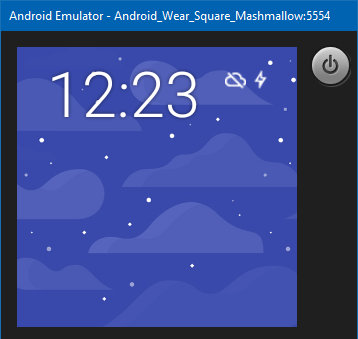
\includegraphics[width=.325\textwidth]{1}
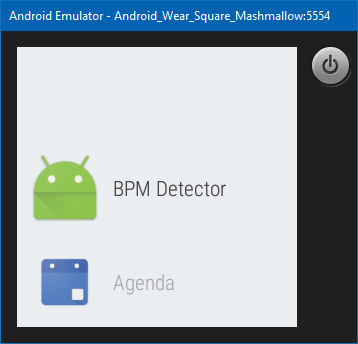
\includegraphics[width=.325\textwidth]{2}
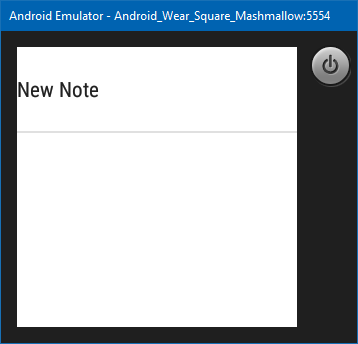
\includegraphics[width=.325\textwidth]{3}
\\\\
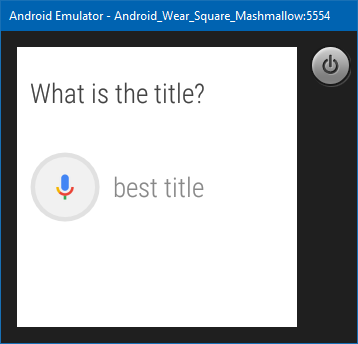
\includegraphics[width=.325\textwidth]{4}
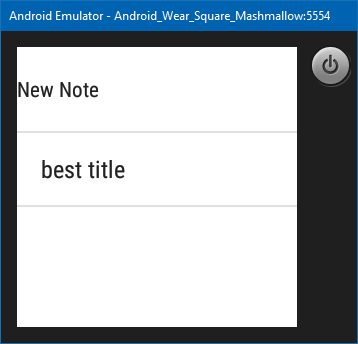
\includegraphics[width=.325\textwidth]{5}
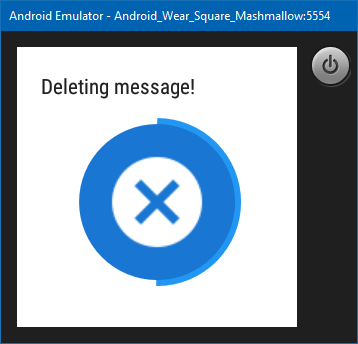
\includegraphics[width=.325\textwidth]{6}
\\\\
After initializing the Android emulator and selecting the application (named "BPM Detector" here), you can select "New Note" where it'll ask "What is the title?" After, the application will save the note, returning you to the main screen where you can make a new note, or delete an existing one by selecting it. If you decide to select a note for deletion, the "Delete message!" screen will appear. Selecting the big X in the middle will cancel the deletion.
\\\\
Android consist of many \textbf{activities}, a component that provides a screen for the user to interact with. Every activity has a method called \textbf{onCreate} which serves as the starting point for it. When switching activities, an \textbf{Intent} is used to describe some operation to perform when making the transition.
\end{figure}

% ========================================================================================================================
\section{Prospective Progress}
\subsection{Overview}
\subsubsection{Continue Learning Android}
Creating the note application was a good introduction to Android development but I will need to continue learning this framework so that I can:
\begin{itemize}
	\item Access the sensors on an Android smartwatch and perform computations to calculate the BPM
	\item Program communications between the smartwatch and the smartphone so that the user can view the BPM in real time
	\item Insert, update, and delete conducting sessions on the smartphone back-end
\end{itemize}
\subsubsection{BPM Testing}
The kinesthetic nature of BPM Detector requires testing the application physically through conducting. To accomplish this, I need to continue repairing my Moto 360 so that I can comfortably develop the GUI on the smartwatch side.

\subsection{Prospective Schedule} 
\begin{center}
  \begin{tabular}{ |c|p{1.6in}|p{4in}| } 
  \hline 
  \multicolumn{3}{|c|}{\textbf{Fall Quarter 2017}} \\
  \hline
  \textbf{Week} & \textbf{Topic} & \textbf{Description} \\ 
  \hline
  1-2 & Back-end & Repair Moto 360. Access smartwatch sensor data to perform BPM computation. \\
  \hline
  3-4 & Back-end & Send computed BPM to smartphone and save the data locally. \\
  \hline
  5 & Front-end & Develop GUI on the smartwatch and smartphone end. \\
  \hline 
  6-7 & Integration & Integrate back-end with front-end. Do this for the smartwatch and smartphone side. \\
  \hline
  8-9 & Integration/Validation Testing & Make sure core BPM detection functionality is working. \\
  \hline
  10 & QA & Polish application, construct final report, and demo. \\
  \hline
  \end{tabular}
\end{center}
Note that tasks may be done during the summer of 2017 to expand the development timeline.  

\newpage

% ========================================================================================================================
\section{Conclusion}
CPE 491 was mainly utilized to set myself up for the main technical implementation. Creating that simple note application provided a solid foundation for me to build on. For the second half of senior project (which will unofficially include summer along side Fall Quarter 2017), I plan to begin programming how the system will calculate the BPM with the sensory data provided by the smartwatch. After the BPM has been calculated, this number must be send back to the smartphone in real time for the front-end. After that is complete, I will need to work on the front-end on both the smartwatch and smartphone side so that the user can view their current BPM along with previous BPMs from past conducting sessions.
\end{document}